
\section{XML and XHTML}

\subsection{W3C Procedure for Recommendation}

The W3C procedure for recommendation is defined as follows: a working group creates a \textit{Working Draft} (which indicates the work in progress). This draft is refined to a \textit{Candidate Recommendation}. The \textit{Candidate Recommendation} is further refined to become a \textit{Proposed Recommendation}. A committee decides on whether or not a \textit{Proposed Recommendation} becomes a \textit{W3C Recommendation}. In between the stages there are rounds for feedback in which people from the community/industry are invited to criticize and help improve the document. This process is represented by image ~\ref{fig:RecommendationProcedure} below.

\vspace{10pt}

\begin{figure}[here]
	\centering
	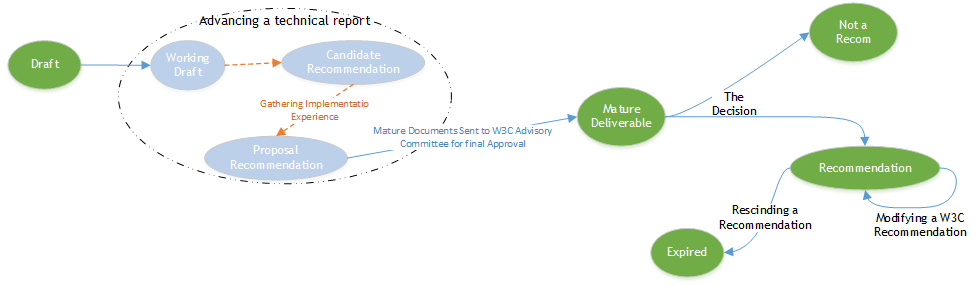
\includegraphics[width=1.0\textwidth]{images/w3c.png}
	\caption{An overview of the W3C Recommendation procedure}
	\label{fig:RecommendationProcedure}
\end{figure}

\subsection{IBM Technical Series}

For this assignment we had to watch three videos that can be found on YouTube:
\begin{itemize}
\item An Introduction to XML: The Basics \citep{ibmtechnicalpart1}
\item An Introduction to XML: XML and Web 2.0 \citep{ibmtechnicalpart2}
\item An Introduction to XML: Managing XML Data \citep{ibmtechnicalpart3}
\end{itemize}


We extracted the following insights from the videos about XML, of which the advantages can be found in table ~\ref{tab:XmlProsCons}. 
\begin{itemize}
\item
XML has a widespread usage everywhere in the industry and is a fully defined, open standard.
\item
It can be used as a meta language (a language describing the language itself).
XML enables easy sharing data between applications, independent of platform or software.
\item
RSS and ATOM allow to syndicate content to users, ATOM features reusable elements while RSS doesn't.
\item
AJAX allows the creation of dynamic web applications.
\item
RDF is the key-language in semantic web development and is XML-based. It describes resources.
\item
XML allows semi-structured or unstructured data, handles nested and complex data, and it's extensible
\item
XQuery and XPath allow to search XML data for specific fields, structures or information
\item
XSLT specifies how to transform XML documents into other XML documents (e.g. applying stylesheet to render XML in browser)
\end{itemize}

\paragraph{Short overview of advantages and disadvantages}
\mbox{}

\begin{table}[h]
\begin{tabular}{|l|l|}
\hline
	\textbf{\color{OliveGreen}Advantages} & \textbf{\color{Maroon}Disadvantages} \\
	\hline
	Widespread usage & Larger size XML records \\
	Platform independent & Implementation cost \\
	Allows for (un)structured data & Higher complexity for retrieval and storage \\
	Self-definable language & \\
\hline
\end{tabular}
\caption{The advantages and disadvantages of XML}
\label{tab:XmlProsCons}
\end{table}


